\chapter{An Isabelle tour, and a first proof or two}

%% sys
%% co
%% figures

\section{Introduction}
Let's take a quick tour of the Isabelle interface, learn a little bit about how to enter text into an Isabelle document, and write a proof of a simple theorem (using tools you won't completely understand because this is a quick tour, not a tutorial). That will give us a chance to see how Isabelle relates to the mathematics you're used to writing. When I use a bit of Isabelle syntax, I'm \textit{not} going to tell you the most general form in which it can be used -- I'll start doing more of that in the next chapter. I say this to warn you that you shouldn't try to generalize too much from what you read here. 
 
This tour will need to introduce things at a bunch of levels -- how do you type that character? What do the colors mean? What kinds of math can I type at \textit{this} point in the file? I'll be answering \textit{some} of the questions at each level, the ones I think are most important for getting started. But you should be prepared to finish the chapter with a lot of unanswered questions.

\subsection{Formatting and style}
The text in this book uses formatting as a guide to content. New terms, for instance, are introduced with \term{this format}. \isi{Isabelle source material} (which I'll also call `code') is in a monospace font with a grey background. Parts of the Isabelle interface like names of \sys{buttons}, menu-options, or panels, have a light-blue/purple background. This is also used for things Isabelle presents as feedback (e.g., the contents of the \sys{Output} panel) except in the rare cases where these are actual Isabelle code. Things related to your computer outside of Isabelle --- directory/folder names, file names like \co{MyTheory.thy}, etc. --- are monospace with a peach background. Because such filenames can also be part of Isabelle code, I won't be completely consistent about this, but I'll try to at least be sensible.

I hope you'll treat reading this book as an \emph{interactive experience}, one where every time you see something new, you'll try it out. To encourage this, I'll sometimes include \term{tasks}, which are things I want you to do right at some particular moment in your reading. The end of a task is marked with a black square. Here's a first one:

\task
As you read this chapter, use Isabelle to do exactly what's described in the text. When I say ``Now delete both \isi{sorry} and the \isi{thm} line,'' you should be editing the text in an Isabelle editor-buffer. Your first step, and the one I am least able to help you with, is to start Isabelle on your computer. 
\etask

Pretty much everything in this book looks the same in Isabelle2023, Isabelle2024, and Isabelle2025, and will probably not change much in the next couple of years. Pick the current latest stable edition of Isabelle, install it, and start it to complete the task. If you're on a Mac, you may have to grant Isabelle various permissions in the Mac's\co{Control Panel...Security} interface to make everything work properly. 

Once you've started up Isabelle, you'll see an interface that looks like this:
\begin{figure}[h]
    \centering
    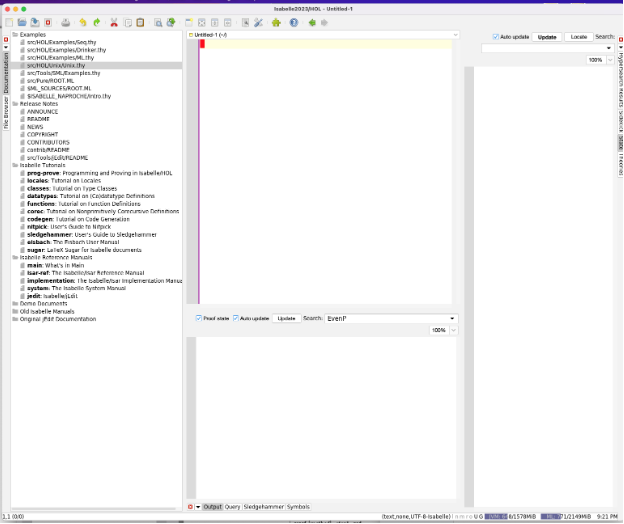
\includegraphics[width=0.7\linewidth]{TEXT//C01//Images/interface.png}
    \caption{The Isabelle interface (as of May 2024)}
    \label{fig:C1-interface}
\end{figure}
In the left column are various documents you can look at. About halfway down, in bold, is \textbf{prog-prove}\textit{\textbf{,}} a book about programming and proving in Isabelle/HOL, which will almost certainly be useful to you at some point, as it is to me. But when I first tried reading it, I rapidly gave up and decided that someone needed to write \textit{this} book instead. 

The top half of the center column is an \sys{Editor} panel -- in it you can type Isabelle documents (which Isabelle folks call \term{theory documents} or \term{proof documents}). As you do so, other threads of execution are constantly processing what you've written and changing the appearance of the editor text -- perhaps color-coding some text, or making red marks along the right-hand side of the document, or generating \textit{output}, which is one of the things that you can see in the other center-column window at the bottom. You can see above that I've got \sys{Output} highlighted; you can actually select \sys{Query}, \sys{Sledgehammer}, or \sys{Symbols} instead. For now, let's stick with \sys{Output}. 

Right here I want to have you do something important. 

\task
Near the top right of the 
\sys{Output} panel, you can see this:
\begin{figure}[h]
    \centering
    
\includegraphics[width=0.75\linewidth]{TEXT/C01//Images/image.png}
\end{figure}
\textit{Be sure that \sys{Proof state} and \sys{Auto update} are both checked.} 
\etask

In everything I write from now on I'll assume that you've done this, so do it now! [Why? Because as you work, you'll constantly be looking at this panel, and having it update as you type, rather than requiring a cursor-motion-and-click, is really nice. Checking \sys{Proof state} says that you'd like to see a little more than the bare minimum feedback, which saves you from looking at \textit{another} panel all the time. As your proof states grow more complicated, you may want to uncheck \sys{Proof state} and use the \sys{State} panel in the third column.]

Moving on, there's the column on the right. \sys{Auto update} is checked, because that's how you'll usually want things -- it means that as you type in the theory document, almost everything in the interface updates accordingly. At the right hand side are choices of what to display in the main panel of that column: \sys{Hypersearch Results}, \sys{Sidekick}, \sys{State}, or \sys{Theories}. For now, we'll go with \sys{State}. Down at the bottom are some bits of information: the current time, how much memory various parts of Isabelle are using, etc. That last item is more important than you might think. Isabelle spawns a lot of processes, and I've found that if I leave Isabelle open on my computer for a few days, it starts slowing down, and a restart of Isabelle often fixes things. One clue to this is when I've done nothing for 6 hours, but the memory usage is some very large number. This shouldn't be a problem for you right now, but it's worth remembering.  

In the middle column, the top panel shows the currently-active file-name at the top (\co{Untitled-1 (\~/)}; if you look to the right of that filename, you'll see a down-arrow that you can click to discover that there may be other editor buffers available for you to look at as well. When I click on mine, I see this:
\begin{figure}
    \centering
    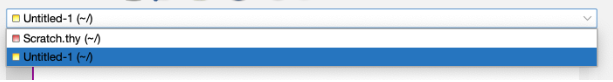
\includegraphics[width=1\linewidth]{TEXT/C01//Images/file-list.png}
\end{figure}
which tells me that in addition to the \co{Untitled-1} document, I also have open a document called \co{Scratch.thy}. By moving my cursor over that file name and releasing, I can switch to showing that document if I like. Using the \sys{File} menu, you can open a new document (it'll be called \co{Unititled-2}) and toggle between the two of them if you like.

In general, dropdowns like this abound. There's another at the top of the lower center panel, and near the top of the right panel. 

It'd be nice to start writing a theorem and proof, but such things must be contained in a \textit{theory file} for Isabelle to process them. So let's save \co{Untitled-1} (type command-S (Mac) or ctrl-S (Windows)) to do so. You'll see a dialog appear. Mine shows that the file will be saved in \co{/Users/jfh}, but I could navigate around to save it somewhere else. It also shows (at the bottom of the dialog box) that the file will be called \co{Untitled-1}:
\begin{figure}[h]
    \centering
    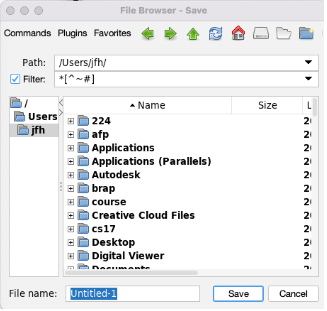
\includegraphics[width=0.5\linewidth]{TEXT/C01//Images/file-chooser.png}
\end{figure}
Let's change that to \co{IBookCh1.thy}, where \co{IBook} means `Isabelle book', \co{Ch1} means `Chapter 1', and \co{.thy} is the extension \textit{required on all theory files}. Without this extension, nothing will work. So let's suck it up and type it in:
\begin{figure}[h]
    \centering
    
\includegraphics[width=0.75\linewidth]{TEXT/C01//Images/file-name-edit.png}
\end{figure}
and click \sys{Save}. 

Two things happen when we save the file: the document title at the top changes to \co{IBookCh1.thy (~/)}, and the cursor in the document becomes bright red:


\begin{figure}[h]
    \centering
    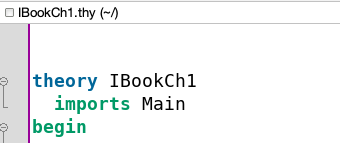
\includegraphics[width=0.5\linewidth]{TEXT/C01//Images/interface-update.png}
\end{figure}
Less obvious is the appearance of a purple line down the left side of the document. 

\digression[File paths]{
The filename above makes sense, but what about the \co{(~/)} after it? In Unix-like operating systems like MacOS, every user has a `home directory' where their files are stored. In my case, that directory is \co{/Users/jfh}. But there's a Unix-standard abbreviation for that, namely a tilde. So \co{\ ~/names.txt} is a way of describing a file called \co{names.txt} that's in my home directory. In the snapshot above, what you're seeing is that there's a file called \co{IBookCh1.thy} in my home directory, the 'directory path' being shown in parentheses at the right. }

\digression[File names]{
The filename may have made sense, but it's not very readable. Why not use some blanks, or hyphens to improve readability? Because those can cause problems for Isabelle. Stick with letters, numbers, and underscores in your file names (except for the \co{.thy} at the end, of course). The Isabelle distribution itself sometimes violates this general rule, and when it does, you have to put double-quotes (\textit{not} smart-quotes!) around the theory name you're importing to prevent problems.} 

We can now start creating our theory document. There are very strict rules for this, rules that I'll enumerate in a little while, but for now, we're just going to type. Here's a start for our theory:

\begin{figure}[h]
    \centering
    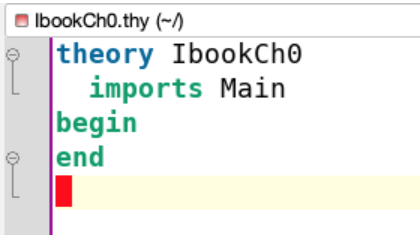
\includegraphics[width=0.5\linewidth]{TEXT/C01//Images/first-theory.png}
    \caption{A first theory document}
    \label{fig:first-theory-doc}
\end{figure}
The theory \textit{must} start with the word \isi{theory}; the theory's name comes next, and it must be exactly the same as the non-extension part of the filename (i.e., the filename except for the \co{.thy} at the end). Then comes the keyword \isi{imports}, and then a \isi{begin-end} pair. Isabelle kindly makes keywords be shown in boldface, and does some automatic indentation for us.  As we add more to our theory, the new material will go between the \isi{begin} and the \isi{end}. I've also put a blank line after the end, and my cursor, highlighted in red, is on that line. 

To the left are two small markers that look like a circle with a `$-$' in it, and then a line with a hook. These represent collapsible parts of the document. If I click on the top circle, the display changes to this:
\begin{figure}[h]
    \centering
    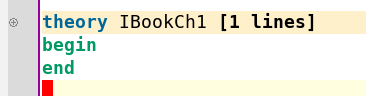
\includegraphics[width=0.5\linewidth]{TEXT/C01//Images/folded-theory.png}
\end{figure}
\noindent which tells you that the first bit of the file has been ``folded up'' and 1 line is now hidden. I can expand it again by clicking on the circled `$+$'. This can be helpful in longer documents for hiding all except the part that you're interested in at some moment. 

\task
Do everything described so far, so that you have your own theory document, and an \isi{imports} line, and a \isi{begin/end} pair,etc.
\etask
By the way, using \isi{imports Main} means that we'll have all sorts of useful facts at our disposal when we want to start writing and proving theorems. An example of this useful stuff is the natural numbers, 0, 1, 2, \ldots  and so on. Those have been defined, and various facts about them proven already, and the theory called \isi{Main} contains these definitions and proofs. (The real and complex numbers are \textit{not} defined in \isi{Main}, by the way; for that you need \isi{Complex_Main}.) You are also allowed to  leave the space after \isi{imports} blank, but you'll find it's hard to do much of anything, because so many important tools are in \isi{Main}.

Every theory file must have an \isi{imports} line. If you want to import more than one theory, you just write them one after another, separated by spaces. So 
\begin{IS}    
imports Main Complex_Main
\end{IS}
\noindent
is also valid. If you typed
\begin{IS}    
imports Main Tigers
\end{IS}    
\noindent
it'd be a problem, though, because there isn't a theory called \isi{Tigers}. Your interface would look like this:
\begin{figure}[h]
    \centering
    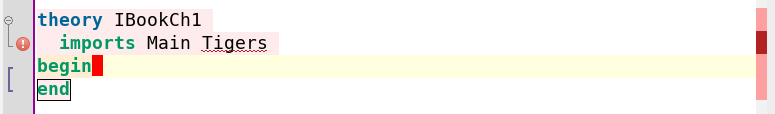
\includegraphics[width=1\linewidth]{TEXT/C01/Images/tigers.png}
\end{figure}
\newpage
And down below, in the Output panel, you'd see this:
\begin{figure}[h]
    \centering
    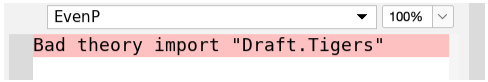
\includegraphics[width=0.75\linewidth]{TEXT/C01/Images/tiger-error.png}
\end{figure}

Or at least you would as long as your cursor was on the \isi{imports} line as shown above. 

What's going on here is that as you're typing, a separate process is interpreting what you've typed, and it's found an error. The red circle with the exclamation point at the left shows the line containing the error. The wiggly red underlining indicates the exact first place the problem occurs. The pink bar to the right with the red rectangle is a schematic picture of your whole document (it's all pink because none of it `works' as a theory file right now), with the location (`near the top') marked with a red bar to tell you where the problem is happening. When your file is 300 lines long, that schematic picture can help you find an error quickly. 

How do you know what theories are available (e.g., \isi{Complex_Main}) and what theories are not (\isi{Tigers})? We'll come back to that. Isabelle has various excellent search tools to help with this kind of question. 

\task
For now, go ahead and get rid of the Tigers so that our theory file is once again valid. 
\etask

\section{A first theorem and proof}
We're now going to state and prove a simple theorem about natural numbers: For any natural number $k$, there's an \textit{even} natural number (i.e., one of the form $2n$) greater than $k$. 

\task I'd like you to pause a moment and think about how you'd prove that. Go ahead and actually write out a proof. (Seriously: do it!) Soon, we'll look at several possible proofs, and chances are good that yours will be among them. 
\etask

To separate that task from my own list of possible proofs, I'll go ahead and talk about how to write this theorem in Isabelle. Between the \isi{begin} and \isi{end} in the theory file, type this: 
\begin{IS}
lemma evens: "\<exists> (n::nat) . 2*n > (k::nat)"
\end{IS}

\marginnote{The non-Isabelle-colored background is there because the isabelle-formatting code used to produce this book converts `\textbackslash\textless exists\textgreater' into the backwards-E, so I had to use a different style.} 
To do this requires writing a 'there exists' symbol, the inverted E. You do that in Isabelle by typing one of three thing ---
\isi{EX} or \verb|\<exists>| or \verb|\exists| --- and then pausing until a tooltip offering up the inverted E as a replacement appears. When it does, hitting TAB will complete the replacement. For this particular example, I've included text, and you can simply copy/paste it into the theory file if you choose to do so.

What does the stuff you just typed \textit{mean}? First, \isi{evens} gives a name to your theorem, which you'll be able to reference later. (Isabelle doesn't require a name, but from force of habit, I always name theorems, and I think it's a good idea.)\marginnote{Often typing some backslash-prepended name will make Isabelle offer \textit{several} replacement options. You can use arrow-keys to move up/down in the list, and then TAB to select one. It appears to me that repeatedly using one replacement will cause it to rise up in the list of choices, at least for a while. This drop-down-to-fill-in thing is hugely useful, but the pause can be annoying. There is some trick for reducing the pause-before-the-list-shows-up, but I cannot seem to find it anywhere in my notes.} Second, \isi{n::nat} means that \isi{n} is a name for something of type \isi{nat}. This \isi{nat} is the \textit{type} (defined somewhere in \isi{Main}) for the natural numbers. So the first bit is saying ``There's a natural number, $n$, \ldots'', and it's followed by a property of that natural number. The division between the name associated with the `there exists' and the property is the period. So now we can read ``There exists a natural number $n$ \textit{such that} $2n$ is greater than the natural number $k$.'' 

Most mathematicians would prefer to say ``for any natural number $k$, there's a natural number $n$ such that $2n > k$,'' and would find the introduction of $k$ at the end of the lemma-statement a bit weird. 

\subsubsection{Consequences}
Your typing that first theorem caused some changes to appear in the interface. Here's what's going on, taken a piece at a time.

First, the color-coding tells you something. A variable associated with an ``exists'' or ``forall'' is said to be a \term{bound variable}, and they show up in green, as happens with $n$ above. Here's another lemma in which \textit{two} variables are bound by a single ``exists'':
\begin{figure}[h]
    
\includegraphics[width=0.5\linewidth]{TEXT/C01/Images/junk-lemma.png}
\end{figure}

\task
Type in this lemma, and observe the changes. 

It's a stupid lemma, but it shows the green highlighting. You can go ahead and delete it now. 
\etask

In the \isi{evens} lemma, the variable k is \textit{unbound}, so it's shown in blue. And a rule in Isabelle is that if a theorem makes a statement like this involving an unbound variable, then once the theorem is proved, the statement is implicitly universally quantified over that variable, so that this lemma (once proved) is really saying ``for any natural number $k$ \ldots'' even though that isn't written down anywhere. There's a sneaky detail about the exact nature of that ``for any'', but I'm going to sweep it under the rug for now. 

Again, while you were typing, another process was interpreting and recoloring. Things now look like this:
\begin{figure}[ht]
    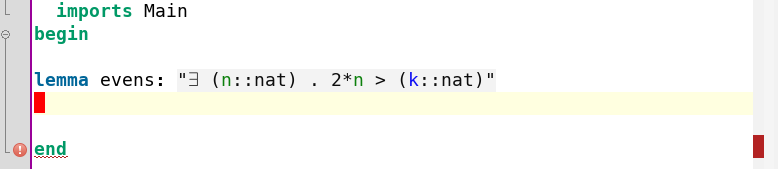
\includegraphics[width=0.75\linewidth]{TEXT/C01/Images/unproved-lemma.png}
\end{figure}
\newpage
(I've trimmed off the top line giving the theory name, and in subsequent images, I'll focus on just the area where we're working.)

The yellow background shows you which line your cursor is on. 

The red exclamation and the red bar at the right tell you something is wrong. Even without looking at the \sys{Output} panel below, you can guess what it is: you've asserted this lemma, but haven't provided a proof. In fact the very act of asserting it put Isabelle in a different mode -- one where it wants a proof, and instead it encountered \isi{end}. The output panel tells you this:

There are three things you can do to address this red stuff in the interface, which generally means something is not right:

\begin{itemize}
    \item Write a proof of the lemma
    \item Give up on the lemma by typing \isi{oops} after it, which says to Isabelle ``I don't know how to prove this, so just forget I ever mentioned it, OK?''  That's useful when you're trying to formulate a statement clearly, but haven't yet worked it out in detail, but also don't want to delete what you've written, \textit{or} have it influence anything that follows. If you were writing a computer program, this would be like "commenting out" a section of your program. 
    \item  (somewhat risky) Assert that you'd like to \textit{pretend} you have a proof, so that you can use this lemma in further work, and you'll get back to proving it properly later. For this, you type \isi{sorry}.
\end{itemize}

Obviously the first of these is the best choice, but sometimes we get frustrated and just need to think some more, so the second is a reasonable option: we get to keep the statement of the theorem there in the file so we don't have to remember how to retype those characters, etc., but it doesn't `pollute' anything. The third is the worst: we treat this unproved thing as if it were true, and use it in subsequent work. Maybe we do this because we're sure we can prove it \textit{eventually}, and this lets us make progress. But it's also possible that we've stated it improperly, and as stated, it's actually false! Then we've effectively introduced a new axiom --- that some false statement is true --- into our system, and from that we can prove anything. That's a terrible thing to do to ourselves. Keep that in mind before you use \isi{sorry.} I give this warning because I've done this exact thing! On the other hand, I also use \isi{sorry} sometimes when I should use \isi{oops}. I'm human, after all. 

\digression[Other uses of \isi{sorry}]{
Sometimes you'll start on a relatively complex proof --- one that involves, say, multiple cases for two different things. The overall \textit{structure} of that proof may be automatically generated as a suggestion for you. It typically involves handling each case separately by proving some small thing; this collection of small proofs amounts to a proof of the main claim. I find it's helpful to get the \textit{structure} all set up, perhaps changing some of the default names that Isabelle has provided to something that better matches my mathematical context, and only \textit{then} work on the details of the proofs. That means that I take the structure, and where it says something like \isi{ then show ?thesis}, I type \isi{sorry} as my proof of that 'thesis'. When I've done this for all the cases, I end up with a 'proof' that would be complete if only I replaced all those \isi{sorry} occurrences with actual proof. 
}

\task 
For now, though, try the experiment. After the lemma, type \isi{sorry}. That word will get highlighted in pink, but you can move on. In fact, you can type \isi{thm evens}, which is a way of asking Isabelle to tell you what it knows about a theorem called \isi{evens}: 
\begin{figure}[h]
    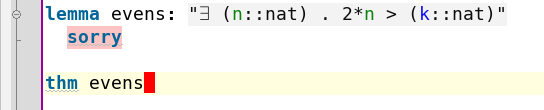
\includegraphics[width=0.75\linewidth]{TEXT/C01//Images/sorry-result.png}
\end{figure}

And down in the \sys{Output} panel you'll get a result:

\begin{figure}[H]
    
\includegraphics[width=0.5\linewidth]{TEXT/C01//Images/result.png}
\end{figure}

That result looks at least somewhat like our theorem. There's a weird question-mark thing going on, and there's no \isi{\\<forall> k} even though I said Isabelle had one implicitly, and the inequality has been swapped around to use \isi{<} instead of \isi{>}, but it's clearly our theorem there on display. All three of these oddities are things that just happen in Isabelle (for good reasons!), and soon you won't notice them as much as you do at first. 

To finish up, go back and remove both the \isi{thm} line and the \isi{sorry} before it.
\etask

We've got a lemma stated, and we need to prove it. 

\subsection{Proving our lemma}
Before we do so, here are some possible proofs:

\begin{itemize}
    \item Just pick $n = k + 1$. It's clearly a natural number, and twice it is obviously larger than $k$ (even in the limiting case where $k$ is zero). 
    \item Consider the cases $k = 0$ and $k > 0$. In the first case, $n = 1$ satisfies $2n > k$. In the second, from $k > 0$ we can add $k$ to both sides to get $2k > k$, so $n = k$ satisfies the theorem.
    \item Induction. Again the case $k = 0$ is trivial. Suppose that for some $k > 0$ we have a number $m$ with $2m > k$. We'll show that there's a number $n$ with $2n > k+1$, thus completing the inductive step. Indeed, it's easy: pick $n = m + 1$. Then $2n = 2m + 2  > k + 2$ (by assumption) which is in turn $> k + 1.$ 
\end{itemize}

Your proof was probably one of these, but there are surely others. If yours was different, by all means try to write it in Isabelle, but don't be frustrated if you cannot do so by the end of this chapter: there's an awful lot you don't yet know. 

For the remainder of this chapter, there's one overarching task: type in everything you see here, observe what happens, then keep reading (possibly deleting something you typed as an experiment). 




Let's see one of Isabelle's strong points right here. We're going to ask it to find a proof, and it's going to try a bunch of strategies --- simplification, 'tableau solvers', a reasoner for linear arithmetic, something called a SAT-solver, etc. --- and see what it can come up with. Typing the word \isi{try} makes all this happen. Sadly, especially for new users, \isi{try} sometimes reports that a proof is easy, but doesn't tell you what to type, which is infuriating. Much nicer is \isi{try0}. So right after our lemma, we'll type \isi{try0} (which dispatches a bunch of processes that report back) and wait for a moment:
\begin{figure}[h]
    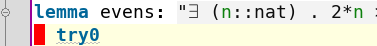
\includegraphics[width=0.5\linewidth]{TEXT/C01//Images/try0.png}
\end{figure}

A moment later, down in the \isi{Output} panel, we see this:
\begin{figure}[H]
    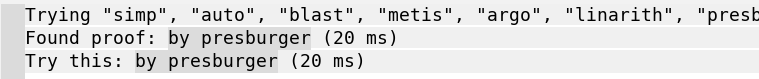
\includegraphics[width=0.75\linewidth]{TEXT/C01//Images/try0-results.png}
\end{figure}

Apparently a proof-method called \isi{presburger} has found a proof. So we can click on the highlighted \isi{by presburger} and it'll be pasted into the buffer. We'll need to backspace out the \isi{try0} to end up with this:
\begin{figure}[h]
    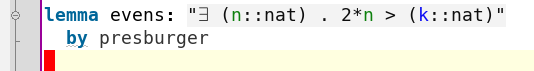
\includegraphics[width=0.5\linewidth]{TEXT/C01/Images/first-proof.png}
\end{figure}
And down in the output window, we have this:
\begin{figure}[h]
    
\includegraphics[width=0.5\linewidth]{TEXT/C01/Images/output-first-proof.png}
\end{figure}

We've got a theorem (stated a little oddly) and it's been proved. We're done! 

We might, however, be unsatisfied. None of us thought up a proof where we just said \isi{by presburger}, right? Maybe we'd like to use one of the proofs that \textbf{we} came up with, so it can be instructive for future students (not to mention being clear!). We'll do that in a moment, but first let's talk about \isi{try0}.

The nice thing about \isi{try0} is that it usually works fast \textit{if} it's going to work at all. And if it \textit{does} work, you can be pretty sure you've stated the theorem correctly. You may still want to work out a different proof, but at least you've got some confidence. The sad thing about \isi{try0} is that sometimes it seems to be unable to prove the most obvious stuff. To be honest, that's usually because you're using it wrong (e.g., you've asked it to prove something false, perhaps by typing less-than-or-equal when you meant less-than). More on this later. 

There's also that question-mark in front of \isi{k}. How did \textit{that} get there, and what does it mean? Again, we'll look at that later.  For now, here's a brief introduction.

You know that $(x^2 - y^2) = (x-y)(x+y)$, right? Knowing that would let Isabelle, during simplification, transform the left side into the right \ldots \textit{literally}  If Isabelle saw $x^2 - y^2$, it could replace it with $(x-y)(x+y)$. On the other hand, if it saw $p^2 - q^2$, it could do nothing. And if it saw $((a+3)^2 - (a+2)^2)$, it could not simplify it to $2a + 5$ using that rule. 

Replacing $x$ and $y$ by \isi{?x} and \isi{?y} says ``this rule can be applied to any pair of \textit{expressions} (of the appropriate type)'', so \isi{?x} could be replaced by $a+3$ and \isi{?y} by $a+2$. (In fact this kind of pattern matching is far more general, but for now, this simple descriptions is enough to get a great deal done.)

\section{Alternative proofs}
Now let's try to do another proof of this theorem. 

\task Copy-and-paste the lemma, and change the name from \isi{evens} to \isi{evens2}. Move your cursor to the next line and wait a moment, and in the \sys{Output} panel, this appears:

\begin{figure}[h]
    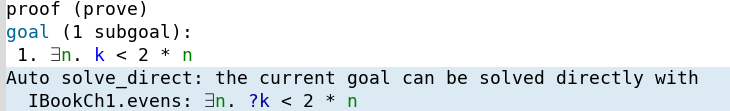
\includegraphics[width=1\linewidth]{TEXT/C01/Images/auto-proof.png}
\end{figure}

Isabelle has done a bit of looking ahead and realized this lemma is particularly easy to prove: it's a consequence of the lemma immediately above (which it has called \isi{IBookCh1.evens}, because we gave it the name \isi{evens}, and it's in a document called \co{IBookCh1.thy}). Unfortunately, it has \textit{not} said how to actually write the proof in Isabelle -- the sort of thing that \isi{try0} might have helped with. It turns out that the magic incantation is \isi{using evens by auto} (although \isi{simp} and \isi{blast} could be used instead of \isi{auto} --- any one of them is capable of making the leap from the statement of \isi{evens} to the statement of \isi{evens2}!) Go ahead and type this to see that you've got a second complete-and-proved lemma.
\etask 

\digression[Proof methods]{Isabelle has several built-in proof methods, tools that help us get from what we know to what we want to prove. Names you'll often see are \isi{auto}, \isi{blast}, \isi{simp}, \isi{metis}, \isi{presberger}. Each is particularly good at one thing. The \isi{simp} method, for instance, is good at a particular standardized form of simplification, as the name suggests\footnote{But while \isi{simp} can do a lot, it doesn't --- without some help and guidance --- handle any kind of algebra with exponents, for example, something most math students do easily in their heads.}. For now we're going to aim to use \isi{auto} as often as possible, but when other names pop up in the next chapter, try to just say to yourself ``I suppose he'll explain what that method does at some point.''
}

Let's try to write one of our \textit{own} proofs of the theorem in Isabelle. Once more, copy-paste the theorem statement and change the name, this time to \isi{evens3}. With your cursor after the theorem, the \sys{Output} panel should now be offering you two ways to trivially prove your theorem, but we're going to ignore those. The \sys{State} panel in the right-hand column is showing this:
\begin{figure}[h]
    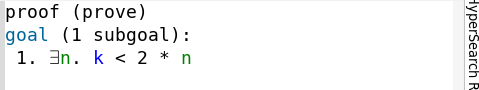
\includegraphics[width=0.75\linewidth]{TEXT/C01/Images/state-panel.png}
\end{figure}

That's telling you a lot. Isabelle has two main modes, `state' and `prove'. (Those are both verbs, not nouns!) In the first, it wants you to state something (which you'll then prove); in the second, it wants you to set about proving one or more things; those things are called \textit{goals} or \textit{subgoals}. In this particular case, we have one goal, which is our current theorem-statement. 

Our prior two proofs are kind of \term{shortcut proofs},  a little bit like when a brief discussion in a textbook concludes with ``we have just shown the following…'', which is followed by some lemma with no further proof. From now on, we're going to mostly avoid those, and our proofs will begin with the word \isi{proof} and end with a matching \isi{qed}. 

To produce the standard kind of proof that we'll generally aim for, we start with the keyword \isi{proof}, followed by something that tells what kind of proof we plan to write (induction, case-analysis, \ldots ). It's also allowable to indicate that we don't have a particular strategy in mind, in which case we write \isi{proof -}. (The hyphen after \isi{proof} is essential! Isabelle expects some proof-method to follow the word \isi{proof}, even if it's something as simple as `no particular method', which is what that hyphen means.)

\textbf{Task}: Add the line \isi{proof -} below your lemma statement and describe how the \sys{Output} and \sys{State} panels have changed. 

We're obliged, at this point, to state something. (Why? Your answer to the previous task should tell you!) We'll generally do so using one of two constructs: \isi{have} and \isi{show}. The \isi{have} construct is for when you want to say something that'll be useful (``$u$ has a unique factorization'') but which isn't one of the current goals. The \isi{show} construct is for when you want to actually establish the truth of some goal (or \term{refine} it -- more on this later). 

Let's commit to one of the proofs, namely the one where we said this:
\begin{quotation}
Just pick $n = k + 1$. It's clearly a natural number, and twice it is obviously larger than $k$ (even in the limiting case where $k$ is zero). 
\end{quotation}
In this case, we're saying that 

\begin{enumerate}
    \item $2(k+1) > k$ (we'll need to prove that), and 
    \item thus there exists a number $n$ with $2n > k$. 
\end{enumerate}
This is a pretty typical situation. We have some proposition (in this case $P(n): 2n > k$), and we want to show that there's some $n$ for which this proposition is true, i.e., we want to show
$$
\exists n . P(n)
$$
We plan to do so by showing that there's a \textit{particular} $n$ for which this is true. (Logicians call this a \term{witness}.) From a logic point of view, we're asserting that
$$
P(b) \implies \exists n . P(n)
$$
And indeed, this is one of Isabelle/HOL's rules for proving things. So let's first establish the truth of the left-hand side here, i.e., exhibit a value of $n$ for which $P(n)$ is true. (We have one in mind, of course -- $k+1$, right?) So we want to say

\begin{IS}
have 2(k+1) > k
\end{IS}
\noindent
i.e., ``we have, as a true-but-yet-to-be-proved fact, that for our natural number $k, 2(k+1) > k.$'' Here \isi{have} is a keyword, and will show up (like \isi{begin} and \isi{end} and \isi{lemma} and other things you've seen) in a bold font in the interface. On the other hand, \isi{"2(k+1) > k"} is not a part of Isabelle's so-called \term{outer syntax}. The general rule is ``stuff like that gets double-quotes'', so we actually have to write
\begin{IS}
have "2*(k+1) > k"    
\end{IS}

\task Go ahead and type that on a line by itself and note the change in the Output and in the State panels. Note: the ``star'' for multiplication is essential. Try deleting it and see what kinds of error messages appear; then replace it. Remember this experience though, because sometime in the future you'll again mis-type something in these double-quotes and get a similar error message, which may seem cryptic until you realize that you need to be really careful in writing math for Isabelle.
\etask

A warning for new Isabelle users: it's \textit{really} easy to forget quotation marks. Here's an example of a small theorem-statement. 
\begin{figure}[h]
    \includegraphics[width=0.5\linewidth]{TEXT/C01//Images/missing_quotes.png}
\end{figure}
The second-to-last line asserts a fact to be shown, but the author has failed to put quotation marks around the fact. Isabelle makes a best-effort at parsing, but at them moment it encounters the not-equal sign, it gives up. I suppose that I still make this mistake on about one in every twenty facts I assert. Sometimes it's because I've copy-pasted, and left off the quotation mark. Sometimes it's forgetfulness. Either way, it's maddening. Start training yourself right now to \textit{always} type those quotation marks!

When we're marshaling facts like the one above (it's not really a `fact' yet because we haven't proved it!) it's nice to give them names. We'll see why in a moment. In this case let's give it the name `example', by writing
\begin{IS}
have example: "2*(k+1) > k"    
\end{IS}

\task 
Try replacing the name ``example'' with ``instance''. What goes wrong? 
\etask

We now have a subgoal to prove, and as it's mere algebra without any exponents, 'simp' can probably handle it.  We add \isi{by simp} on the next line, and see what happens. The \sys{Output} now looks like this:

\begin{figure}[h]
    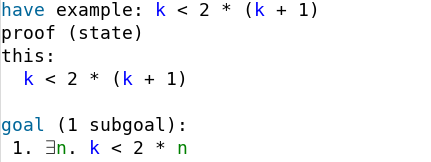
\includegraphics[width=0.5\linewidth]{TEXT/C01/Images/proof-state.png}
\end{figure}

We have a fact called \isi{example}; the current state of things is that we know a fact (the most recent fact is called \isi{this}), and we have a \textit{goal} that we still haven't proved, so we're obliged to do so. With our fact in hand, this \textit{should} be easy. (Note, by the way, that Isabelle has reversed the direction of the inequalities; it always replaces greater-than with less-than!)

This time, we want to assert the overall goal as the next thing to prove, and because we're demonstrating the proof of some \textit{goal}, we use \isi{have} instead of \isi{show}. We \textit{could} retype the overall goal (or copy-paste it from the output panel!) as in 
\begin{figure}[h]
    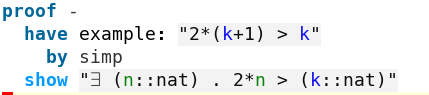
\includegraphics[width=0.5\linewidth]{TEXT/C01/Images/bad-show.png}
\end{figure}

But it's more idiomatic to write this:
\begin{figure}[H]
    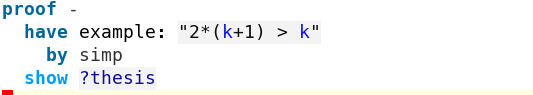
\includegraphics[width=0.75\linewidth]{TEXT/C01/Images/good-show.png}
\end{figure}

That \isi{?thesis} is shorthand for ``the thing we promised to prove'', more or less. (more precisely, it's the thing we promised to show before the most recent \isi{proof -} line). 

We can complete the proof with \isi{using example by blast}. The \isi{using} adds the fact we called \isi{example} to the set of things Isabelle can work with, and \isi{blast} is a prover that does reasoning that includes things like $P(a) \implies \exists x . P(x)$.

A challenge for beginning Isabelle-users is figuring out ``by WHAT???'', because there's \isi{simp}, \isi{auto}, \isi{blast}, \isi{metis}, \ldots  and (a) each of them overlaps with the others to some degree and (b) the names don't really disclose what each one does unless you know more about logic-and-computation than do most mathematicians. I confess that I often use \isi{try0}, so in this case I'd type \isi{using example try0}. The result is a flood of successful proofs:
\begin{figure}[h]
    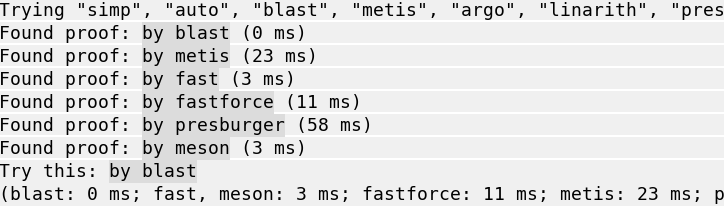
\includegraphics[width=0.75\linewidth]{TEXT/C01/Images/flood.png}
\end{figure}

You can see that this is an easy problem for \isi{blast}, and harder for \isi{fastforce}, and even harder for \isi{presburger} (indeed, that last approach is probably ignoring our 'example' fact and just proving the whole theorem from scratch as it did in the first lemma, \isi{evens}).

And while I \textit{do} use \isi{try0}, I also try to \textit{avoid} using it and get a feel for which solver is the `right' one, as I did when using \isi{simp} to show that $2*(k+1) > k.$ 

So now we have a complete proof:
\begin{figure}[h]
    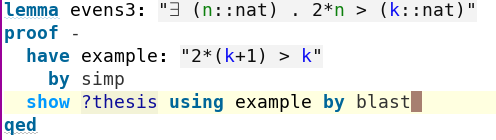
\includegraphics[width=0.75\linewidth]{TEXT/C01/Images/proof1.png}
    \caption{Our first complete proof!}
    \label{fig:first-proof}
\end{figure}

With the cursor in the position shown, the \sys{Output} panel now announces \sys{No subgoals!} and we can add \isi{qed}, which is like a closing-parenthesis for \isi{proof}. If you move your cursor up and down through the proof, you can see how the output changes after each line. 

You will soon grow to love seeing \sys{No subgoals!} It's like being able to check an item off your list of things you need to do -- it feels good! And just as some people enjoy that so much that they begin adding tiny tasks (`Find shovel') to the list before larger ones (`Shovel snow off driveway'), you may find yourself so eager to see \sys{No subgoals!} that you begin proving small things on the way to larger ones. Fortunately, this is an \textit{excellent} strategy in Isabelle. 

Returning to the lemma we're working on, if you change the method used to show \isi{?thesis}, something a bit surprising happens. Change \isi{blast} to \isi{auto} (which cannot in fact do the proof) and you'll once again see that there are no goals left. But something critically important has happened -- red error bars appear on the right-hand side, indicating that this is a place where problems remain. Furthermore, down in the \sys{Output} panel there's an error message telling you that no proof was found. 

What's going on here is that there are multiple threads of execution interacting with this UI, and at least one of them is saying, ``Well, if you say that you've shown something, I guess I'll trust you'' and says that there are no further goals. Another thread might be off looking for a proof of that claim, and simply not have finished the job. (In our case it \textit{has} finished and failed to find a proof, but the idea's the same.) This somewhat peculiar behavior can be both a benefit and a curse. You should get accustomed to looking at those red or pink bars on the right to be sure things have gone as well as you might think that they have. 

Speaking of that, when you load a big theory file -- hundreds of lines perhaps -- you'll see a pink bar at the right indicating that Isabelle has not checked the theory for correctness. Soon the top of that bar will turn white --- Isabelle has checked the part that's visible in the editor panel. As you move your cursor down in the editor, more and more will turn white unless you encounter an error or a place where the proving takes a while to complete. 
\digression[Pre-compiled theories]{ If the theory file is a big one, this might take a while. You can move your cursor to the end of the file and watch the pink stuff gradually disappear --- a good time to get a cup of coffee! --- or you can do this waiting just once, and then \textit{save} the results so that the file (with all its already-checked proofs) can be loaded almost instantly the next time. After several years of proving, I'm just now reaching the situation where that sort of `save-the-results' seems worthwhile, partly because my work is an accumulation of things, and I sometimes find myself wanting to change something early in the work, so a re-compilation ends up being necessary, so the time-savings isn't really so great.}

\subsubsection{Two more proofs}

We have two more proofs of our lemma still waiting in the wings. Here they are, encoded in Isabelle, for you to look at. I'm not going to explain them in the same detail as the first proof, but you should type them in and step through them, watching how the proof-state changes with each line, as a way of getting a feel for two other proof strategies. 

By the way, none of the proofs in this chapter should be considered models of compactness or excellent style. They're straightforward and somewhat wordy and show some basic Isabelle tools using only a few keywords, and that's intentional. I want to set you up to be able to construct a few more proofs of simple statements on your own. They also follow some conventions like 

\begin{itemize}
    \item Using names for facts, particularly long names
    \item Annotating with "(*" and  "*)" comments to explain what's going on; usually Isabelle proofs aim for brevity rather than readability.
\end{itemize}

To continue with our small theorem, we have two more proofs: 

\begin{quotation}
Consider the cases $k = 0$ and $k > 0$. In the first case, $n = 1$ satisfies $2n > k$. In the second, from $k > 0$ we can add $k$ to both sides to get $2k > k$, so $n = k$ satisfies the theorem.
\end{quotation}

Here's that proof\footnote{In both of these proofs, the keyword \isi{next} appears. It's used when there are multiple goals (typical of a proof by cases) or in induction, where the `base case' and `inductive case' are two separate goals. We'll return to exactly how it's used later.}

, in Isabelle:
\begin{figure}[h]
    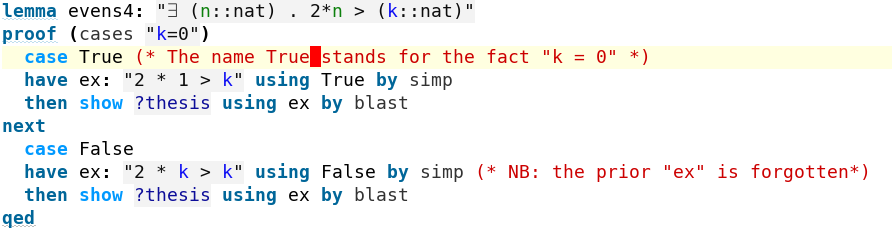
\includegraphics[width=1\linewidth]{TEXT/C01/Images/proof2.png}
    \caption{A proof by cases}
\end{figure}

\begin{quotation}    
Induction. Again the case $k = 0$ is trivial. Suppose that for some $k > 0$ we have a number $m$ with $2m > k$. We'll show that there's a number $n$ with $2n > k+1$, thus completing the inductive step. Indeed, it's easy: pick $n = m + 1$. Then $2n = 2m + 2  > k + 2$ (by assumption). This is in turn $> k + 1.$ 
\end{quotation}

The proof, in Isabelle:

\begin{figure}[ht]
    \centering
    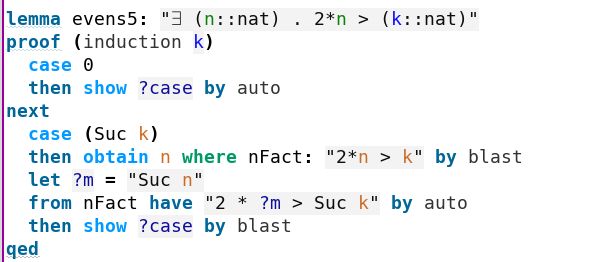
\includegraphics[width=0.75\linewidth]{TEXT/C01/Images/proof3.png}
    \caption{A proof by induction}
\end{figure}


If that last proof looks only superficially like induction to you, you're in good company. You can certainly see that things fall into a base case and an inductive case, and the ``assume $P(k)$'' part of things is somehow all automatically laid out by saying \isi{case (Suc k)}. The rest probably feels just a bit weird, and that's OK. For instance, we no longer have \isi{show ?thesis} but instead \isi{show ?case}. 

Induction in Isabelle is very general and very powerful, but is therefore also a little challenging to use in simple cases, and pretty inscrutable to the beginner.

We've also used \isi{obtain} here. Remember how I said that there's a rule $P(b) \implies \exists x . P(x)$, so that writing down one example for which $P$ is true suffices to show the ``there-exists'' claim? The word \isi{obtain} is the counterpoint to that: it says  that if you know there's an $x$ with $P(x)$ being true, then you can create a name for such an $x$ and use it in the rest of your proof. As an example, the intermediate value theorem says that if $f$ is a continuous function from the reals to the reals and $f(0) > 0$ and $f(1) < 0$, then $f(x) = 0$ for some $x$ between $0$ and $1$. If we'd proved this theorem in Isabelle, we could write \isi{obtain c where "f(c) = 0"} and use \isi{c} in the remainder of some proof.  

\section{Review}
Let's review a few key points from this chapter:

\begin{itemize}
    \item The UI has three panels -- the editor, the proof-state, and the output -- that you'll use a lot while creating theory files

\begin{itemize}
        \item Color-coding and automatic formatting of text tell you a \textit{lot} about what's going on
        \item There are multiple processes acting on the UI at any moment, and their interaction can occasionally be surprising. 
        \item \textit{\textit{Always} pay attention to anything that's red!}
\end{itemize}

    \item Theory-files have a fixed structure; the name of the theory must match the name of the file; the name of the file must end in \isi{.thy}, and the theory name should contain only letters, digits, and underscores. 
    \item Isabelle uses a lot of special symbols. You've learned how to type one of them using the ``type something, pause, and then hit TAB'' approach, but you'll need to learn more. 
    \item Theory-files have a block structure: each \isi{proof} must be matched by a \isi{qed}; each \isi{begin} must be matched by an \isi{end}
    \item If you can't prove something, \isi{oops} is a good way to tell Isabelle to forget all about it. \isi{sorry} is a less-good way, but frequently useful.
    \item Non-keyword text in an Isabelle document generally needs double quotation marks around it. (We'll learn later to use `cartouches' as an alternative.)
    \item You've seen two forms of proof, one of which omits the word \isi{proof} and simply says something like \isi{by auto}; the other one starts with \isi{proof} and ends with \isi{qed}
    \item Within proofs, there are various 'proof methods' named \isi{simp, auto, blast, metis}, etc., that are good at different things, and you'll need to learn which ones are good at which things. For now, that's just a big pile of words. 
    \item When you're in a state of affairs that requires a proof (the proof-state panel says \sys{proof (prove)}), you can type \isi{try} or (better in general) \isi{try0} to see whether Isabelle can find an easy proof for you. 
    \item Proofs can have various structures (cases, contradiction, induction, \ldots ) and each has its own way of being written in Isabelle. 
    \item During a proof, there are goals and subgoals, and your aim is to eliminate all of them. 
    \item You've learned about quite a few Isabelle keywords -- \isi{theory}, \isi{imports}, \isi{begin}, \isi{end}, \isi{lemma}, \isi{using}, \isi{by}, \isi{proof}, \isi{have}, \isi{show}, \isi{case}, \isi{let}, \isi{obtain} -- although the details of most are still to be disclosed. 
    \item You're ready to do some proofs on your own as homework or better, as ``drill'' to help get some patterns into your head. 
\end{itemize}

Finally, I want to note that absolutely nothing we've done so far matches a typical use of Isabelle by an expert -- an expert would have started out any project by searching through Isabelle's known theorems (using its powerful search tools!) to see whether the thing they're trying to prove is already known, or at least something \textit{similar} is known and can be used as a starting point. We'll get to this kind of proving later. 

\section{Homework Exercises}

\begin{enumerate}
    \item Create a new theory file to hold a theory called HW1. What should the name of the file be? Make sure to follow the naming rules.
    \item Type enough into the file to make it a valid theory file (i.e., something beginning with the word \isi{theory} and ending with \isi{end}, and having all keywords highlighted by Isabelle.)
    \item Here's a tiny theorem: \textit{For any natural number n, there's an odd number larger than n. }And here's a proof:\textit{ The number 2n + 1 is an odd number larger than n. }

State and prove this theorem (using the proof above), in Isabelle, using a proof that starts with the word \isi{proof} rather than just \isi{by}. Try to do it without using \isi{try} or \isi{try0}. Call your theorem \isi{odds}. 

\item Change the first word of your theorem statement from \isi{theorem} to \isi{lemma} or vice versa to see that the results are identical. The word \isi{proposition} can also be used. 
 
\item Here's another theorem: The square of any natural number is nonnegative. State and prove this in Isabelle. To write the square of a number \isi{b}, for now just use \isi{b * b}. Hint: to get the ``greater-than-or-equal'' symbol, type `\textbackslash{}ge' and pause until a completion/substitution is offered, and then press TAB. And to indicate that $n$ is a natural number, use \isi{n::nat}, which must be in parentheses to make parsing work. Go ahead and use a \isi{by} proof, because you don't yet know how to find a theorem that says that the product of non-negatives is non-negative, or that naturals are closed under multiplication, but both are true and known within \isi{Main}. Looking at the hints provided by \sys{Auto solve\_direct} will give you some feel for the kinds of facts that are available to you. 
\end{enumerate}

\section{Lagniappe}

Just as the red circle with an exclamation in the left edge of a theory document signals an error, a blue circle with an ``i'' in it tells you that Isabelle has something you might want to know, like the fact that \isi{evens2} was easily proved using the \isi{evens} lemma. 

 
